\documentclass[64pt,aspectratio=169]{beamer}
\usetheme{mpiisimple}
\usepackage{pdfcomment}
\usepackage[utf8]{inputenc}
\usepackage{graphicx}
\usepackage{amsmath,amsfonts,amssymb,amsthm}
\usepackage{tikz}

\title[Robustness and Uncertainty in Deep Learning]{Understanding and Improving Robustness and Uncertainty Estimation in Deep Learning}

\begin{document}
	\begin{frame}[noframenumbering]
		\vskip 0.2cm
		\begin{minipage}{\textwidth}
			\huge\bfseries
			{Understanding and Improving}\\
			Robustness and Uncertainty Estimation\\[0px]
			{in Deep Learning}
		\end{minipage}
		\vskip 0.35cm
		
		\begin{center}
			\begin{minipage}[t]{0.32\textwidth}
				\centering
				\begin{tikzpicture}
					\clip (0,0)  circle (2cm);
					\node[anchor=center] at (0,0) {
\includegraphics[width=2.75cm]{assets/cvpr2019_topic}};
					\draw[draw=MPIIblack] (0,0) circle (2cm);
				\end{tikzpicture}
			\end{minipage}
			\begin{minipage}[t]{0.32\textwidth}
				\centering
				\begin{tikzpicture}
					\clip (0,0)  circle (2cm);
					\node[anchor=center] at (-0.25,0) {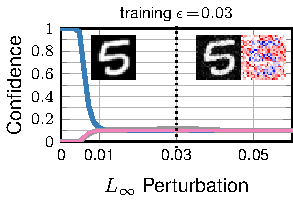
\includegraphics[width=4cm]{assets/icml2020_topic}};
					\draw[draw=MPIIblack] (0,0) circle (2cm);
				\end{tikzpicture}		
			\end{minipage}
			\begin{minipage}[t]{0.32\textwidth}
				\centering
				\begin{tikzpicture}
					\clip (0,0)  circle (2cm);
					\node[anchor=center] at (-0.5,0) {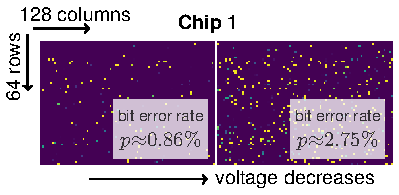
\includegraphics[width=5.33cm]{assets/tpami2022_topic}};
					\draw[draw=MPIIblack] (0,0) circle (2cm);
				\end{tikzpicture}
			\end{minipage}
		\end{center}
		\vskip 0.2cm
		
		{\large Name -- PhD Defense Talk -- Date}
		\vskip 0.25cm
		
		
\includegraphics[height=0.65cm]{assets/logos/mpilogo-inf-wide}
		\hspace*{0.35cm}
		
\includegraphics[height=0.65cm,clip,trim={0 0 6cm 0}]{assets/logos/sic}
		\hspace*{0.35cm}
		
\includegraphics[height=0.65cm]{assets/logos/uds}
		
		\marginnote{\pdfcomment[icon=note]{
				Notes for use with pdfpc.
		}}
	\end{frame}
	
	\setbeamertemplate{footline}{
		\begin{textblock*}{\paperwidth}(4mm,84mm)
			\hfill
			\begin{minipage}{8mm}
				\color{MPIIdarkgray}\small\raggedleft\insertframenumber
			\end{minipage}
			\hspace*{7mm}
		\end{textblock*}
	}
	
	\addtocounter{framenumber}{-1}
	\begin{frame}{Safety-Critical Deep Learning}		
		\Large 
		\centering
		
		Slide with footer
	\end{frame}
	
	\begingroup
	\setbeamertemplate{footline}{}
	\begin{frame}[noframenumbering]{}
		\Large
		
		\vspace*{-0.2cm}
		\begin{minipage}{0.27\textwidth}
			\bfseries\huge Questions?
		\end{minipage}
		\hfill
		\begin{minipage}{0.01\textwidth}
			{\color{gray}\rule{0.5pt}{1.5cm}}
		\end{minipage}
		\hfill
		\begin{minipage}{0.7\textwidth}
			\color{gray}
			Understanding and Improving
			Robustness and\\
			Uncertainty Estimation
			in Deep Learning
		\end{minipage}
		\vskip 0.35cm
		
		\begin{center}
			\begin{minipage}[t]{0.22\textwidth}\vspace*{0px}
				\centering
				\begin{tikzpicture}
					\clip (0,0)  circle (1.5cm);
					\node[anchor=center] at (0,0) {
\includegraphics[width=2.125cm]{assets/cvpr2019_topic}};
					\draw[draw=MPIIblack] (0,0) circle (1.5cm);
				\end{tikzpicture}
			\end{minipage}
			\begin{minipage}[t]{0.22\textwidth}\vspace*{0px}
				\centering
				\begin{tikzpicture}
					\clip (0,0)  circle (1.5cm);
					\node[anchor=center] at (-0.05,0) {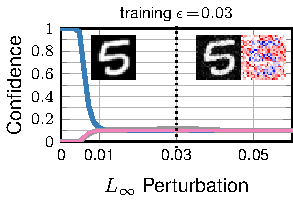
\includegraphics[width=3cm]{assets/icml2020_topic}};
					\draw[draw=MPIIblack] (0,0) circle (1.5cm);
				\end{tikzpicture}		
			\end{minipage}
			\begin{minipage}[t]{0.22\textwidth}\vspace*{0px}
				\centering
				\begin{tikzpicture}
					\clip (0,0)  circle (1.5cm);
					\node[anchor=center] at (-0.4,0) {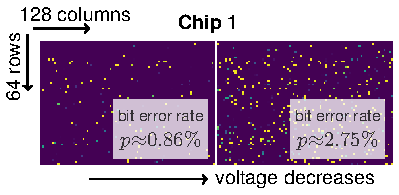
\includegraphics[width=4cm]{assets/tpami2022_topic}};
					\draw[draw=MPIIblack] (0,0) circle (1.5cm);
				\end{tikzpicture}
			\end{minipage}
			\hfill
			\begin{minipage}[t]{0.31\textwidth}\vspace*{0px}
				\small
				\vspace{0.1cm}
				\underline{Committee:}\\
				Member 1\\
				Member 1\\
				Member 1\\
				Member 1\\
				Chair (chair)\\
				Academic assistant (assist.)
			\end{minipage}
		\end{center}
		
		{\large Name -- PhD Defense Talk -- Date -- \url{webpage.com}}
		
		\vfill
		
\begin{tikzpicture}
			\draw (0, 0) rectangle (8, 1.75);
			\node[anchor=west] at (0, 0.9){Placeholder for images};
		\end{tikzpicture}
		
		\vfill
		
\includegraphics[height=0.65cm]{assets/logos/mpilogo-inf-wide}
		\hspace*{0.35cm}
		
\includegraphics[height=0.65cm,clip,trim={0 0 6cm 0}]{assets/logos/sic}
		\hspace*{0.35cm}
		
\includegraphics[height=0.65cm]{assets/logos/uds}
		\vspace*{-0.5cm}
	\end{frame}
	\endgroup
\end{document}
